% Provenance (never printed): old premiere S / seconde material on minerals and
% rocks (identifying minerals in hand specimen, the silicates, the minerals of
% granite, basalt and peridotite, thin sections in polarised light).
% Element fractions and rock densities from figdata/grade-11/mineral_density.py
% (Rudnick and Gao 2014 bulk crust; webmineral mean densities). Mineral, crystal,
% rock families and the Mohs scale are Book 1's (grade 6): recalled, not defined.
% Felsic and mafic belong to g11.08: not used here.
\chapter{矿物}\label{ch:g11:minerals}

拿起一块花岗岩卵石，用手持放大镜观察。它并不是单一物质，
而是由许多颗粒紧密嵌合而成的集合体：灰色颗粒，玻璃质，几乎透明；
粉红色颗粒，呈块状，转动卵石时，其断面在光下闪闪发亮；
细小的黑色\omterm{def:g11:minerals:thin-section}{薄片}，用刀尖即可挑成薄层。
每一种颗粒都是一种矿物。本章说明地质学家如何区分它们，
为何它们几乎都由硅和氧构成，
以及它们如何构成前面已接触过的岩石——花岗岩、玄武岩、
\omterm{def:g11:ocean-ridges:peridotite}{橄榄岩}——还有一片比头发丝还薄的岩石\omterm{def:g11:minerals:thin-section}{薄片}
在偏光下如何同时呈现它们。

\begin{omfigure}
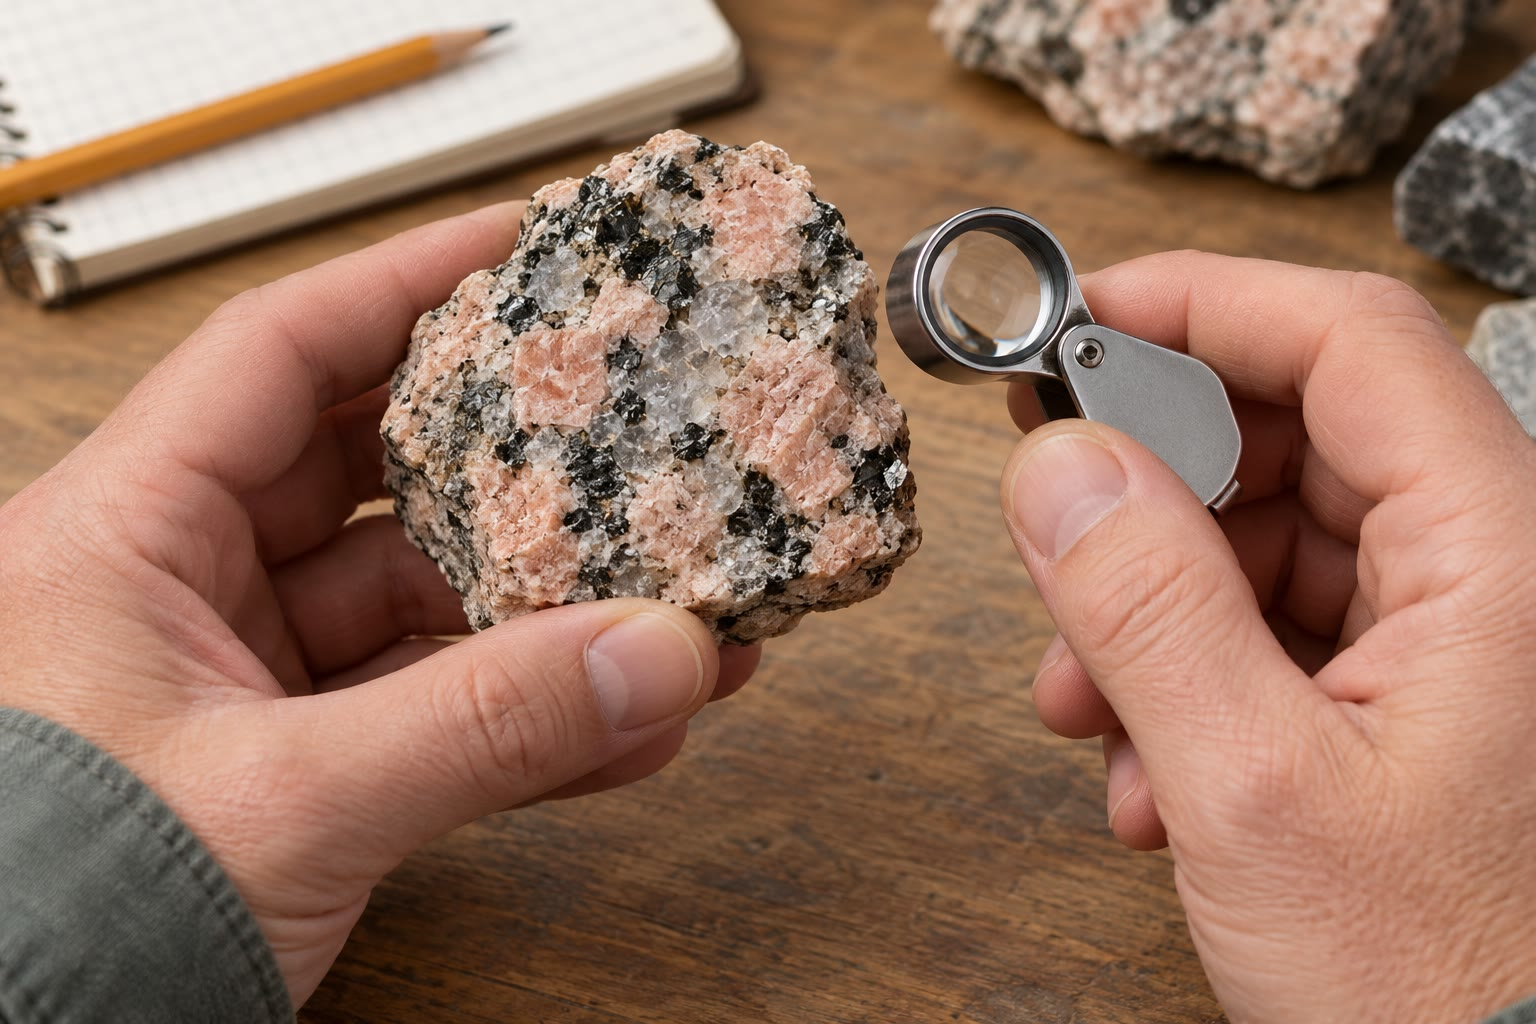
\includegraphics[width=0.62\linewidth]{images/book2/ai/g11-geologist-hand-lens.jpg}

{\small 用手持放大镜观察花岗岩：区分矿物的第一件工具。
（AI 生成插图。）}
\end{omfigure}

\begin{recall}
矿物是天然形成的固体物质，并非由生物制造，
具有固定的化学组成，原子呈规则排列；岩石由一种或几种矿物组成。
花岗岩主要由长石、石英和云母组成。
岩石分为三大类：火成岩、沉积岩和变质岩。
矿物的硬度是指其抵抗刻划的能力，按莫氏硬度表从 1
（滑石）到 10（金刚石）分级；正长石为 6，石英为
7，玻璃片约为 5.5，钢钉约为 6.5（第 1 册，
六年级）。物体的密度等于其质量除以体积
（物理学）。化合物可用化学式表示，化学式给出其原子个数；在
由离子构成的固体中，正负电荷相互平衡（化学）。
\omterm{def:g11:ocean-ridges:peridotite}{橄榄岩}构成地幔；\omterm{def:g11:ocean-ridges:gabbro}{辉长岩}和玄武岩构成\omterm{def:g11:ocean-ridges:oceanic-lithosphere}{洋壳}
（见\cref{ch:g11:ocean-ridges}）。
\end{recall}
% ledger: usgs:mineral-rock, nps:granite-minerals, nps:mohs-ladder, nps:mohs-testers

\section{区分矿物}

矿物具有固定的化学组成和规则的原子排列，两者都能
从外部表现出来：晶体的形状、断裂方式、
反射光线的方式、硬度和密度。这些性质单独
都不足以确定矿物；合在一起，便可在手标本中辨认常见矿物，
不借助仪器，只需放大镜、钢钉和玻璃片。

\paragraph{形状。}晶体若在空洞或液体中自由生长，
其形状便反映原子的排列方式。

\begin{definition}[晶习]\label{def:g11:minerals:habit}
矿物的\emph{晶习}\index{晶习（晶体的）}是指
其晶体所呈现的一般形状：立方体状、板状（扁平，如平板）、柱状
（细长，如棱柱）、刀片状、针状（似针）等。
\end{definition}
% ledger: tulane:physprop

石英呈六方柱状生长，末端为尖顶；黑云母则呈扁平的
六边形片状（见下方照片）。然而在多数岩石中，颗粒彼此
挤压生长，没有自身的晶面，此时\omterm{def:g11:minerals:habit}{晶习}提供的信息很少，
其他性质便起主要作用。
% ledger: photo:g11-quartz, photo:g11-biotite

\paragraph{颜色与\omterm{def:g11:minerals:lustre}{光泽}。}颜色是人们最先看到的特征，也是
最不可靠的。仅含少量其他元素便足以改变颜色：石英
可呈无色透明、白色、黑色、粉红色、蓝色或紫色。另有一些矿物
则几乎不变：橄榄石几乎总是绿色的。矿物如何
反射光线，是更好的判别依据。
% ledger: tulane:physprop

\begin{definition}[光泽]\label{def:g11:minerals:lustre}
矿物的\emph{光泽}\index{光泽}是指其在反射光下所呈现的
外观。矿物像金属一样发亮时，称为\emph{金属光泽}，否则为非金属光泽：
\emph{玻璃光泽}（像玻璃，如石英）、珍珠光泽、
树脂光泽等。
\end{definition}
% ledger: tulane:physprop

\paragraph{断裂方式。}敲击晶体，它便会断开。若
其原子间的化学键在某些面上较弱，便沿这些面裂开，
反复裂开，形成平坦而发亮的表面；若没有任何面比其他面更弱，
则沿任意表面断裂。

\begin{definition}[解理；断口]\label{def:g11:minerals:cleavage}
\emph{解理}\index{解理（矿物的）}是指矿物
沿平坦平面断裂的趋势，这些平面平行于其原子间键较弱的方向。
\emph{断口}\index{断口（矿物的）}是指
在无弱面的矿物中沿不规则表面发生的断裂；
断面光滑、呈弧形、如破碎玻璃一般的断口，
称为\emph{贝壳状}。
\end{definition}
% ledger: tulane:physprop

矿物可能具有一组、两组、三组\omterm{def:g11:minerals:cleavage}{解理}，也可能没有。云母具有一组完全\omterm{def:g11:minerals:cleavage}{解理}，
能剥成\omterm{def:g11:minerals:thin-section}{薄片}。长石具有两组\omterm{def:g11:minerals:cleavage}{解理}。石英没有\omterm{def:g11:minerals:cleavage}{解理}：它以
贝壳状\omterm{def:g11:minerals:cleavage}{断口}断裂，因而可与颜色相同的灰色或白色长石
立即区分开来。两组\omterm{def:g11:minerals:cleavage}{解理}之间的夹角由原子排列决定，
可在断裂的颗粒或切面上测量：
辉石的两组\omterm{def:g11:minerals:cleavage}{解理}的夹角约为\ang{87}和\ang{93}，接近直角；
角闪石的则约为\ang{56}和\ang{124}。辉石与角闪石
常为深色且外观相似，\omterm{def:g11:minerals:cleavage}{解理}夹角可以将二者区分开来。
% ledger: wm:densities (quartz conchoidal; orthoclase two cleavages; biotite one), tulane:cleavage-angles

\begin{omfigure}
\begin{tikzpicture}[font=\footnotesize]
  % pyroxene: octagonal cross-section, cleavage traces at 46.5 and 133.5 degrees (87/93)
  \begin{scope}
    \coordinate (p1) at (1,0.4); \coordinate (p2) at (0.431,1); \coordinate (p3) at (-0.431,1);
    \coordinate (p4) at (-1,0.4); \coordinate (p5) at (-1,-0.4); \coordinate (p6) at (-0.431,-1);
    \coordinate (p7) at (0.431,-1); \coordinate (p8) at (1,-0.4);
    \begin{scope}[scale=1.5]
      \fill[black!72!green!40] (1,0.4) -- (0.431,1) -- (-0.431,1) -- (-1,0.4) -- (-1,-0.4) -- (-0.431,-1) -- (0.431,-1) -- (1,-0.4) -- cycle;
      \clip (1,0.4) -- (0.431,1) -- (-0.431,1) -- (-1,0.4) -- (-1,-0.4) -- (-0.431,-1) -- (0.431,-1) -- (1,-0.4) -- cycle;
      \foreach \s in {-5,...,5} {
        \draw[white!85!black, line width=0.5pt] ($(136.5:\s*0.24)+(46.5:-3)$) -- ($(136.5:\s*0.24)+(46.5:3)$);
        \draw[white!85!black, line width=0.5pt] ($(223.5:\s*0.24)+(133.5:-3)$) -- ($(223.5:\s*0.24)+(133.5:3)$);}
      \draw[black!80, line width=0.9pt] (46.5:-3) -- (46.5:3); \draw[black!80, line width=0.9pt] (133.5:-3) -- (133.5:3);
    \end{scope}
    \draw[black!70, line width=0.7pt, scale=1.5] (1,0.4) -- (0.431,1) -- (-0.431,1) -- (-1,0.4) -- (-1,-0.4) -- (-0.431,-1) -- (0.431,-1) -- (1,-0.4) -- cycle;
    \draw[omProp, line width=1pt] (46.5:0.75) arc[start angle=46.5, end angle=133.5, radius=0.75];
    \draw[omDef, line width=1pt] (133.5:0.5) arc[start angle=133.5, end angle=226.5, radius=0.5];
    \node[fill=white, inner sep=1pt, text=omProp!80!black] at (90:0.98) {\ang{87}};
    \node[fill=white, inner sep=1pt, text=omDef] at (180:0.82) {\ang{93}};
    \node[anchor=north, align=center] at (0,-1.7) {\strut\textbf{辉石}\\解理约为\ang{87}和\ang{93}};
  \end{scope}
  % amphibole: elongated hexagon, cleavage traces at 28 and 152 degrees (56/124 opening sideways)
  \begin{scope}[xshift=6.2cm]
    \begin{scope}[scale=1.5]
      \fill[black!72!green!40] (1.6,0) -- (0.62,0.52) -- (-0.62,0.52) -- (-1.6,0) -- (-0.62,-0.52) -- (0.62,-0.52) -- cycle;
      \clip (1.6,0) -- (0.62,0.52) -- (-0.62,0.52) -- (-1.6,0) -- (-0.62,-0.52) -- (0.62,-0.52) -- cycle;
      \foreach \s in {-6,...,6} {
        \draw[white!85!black, line width=0.5pt] ($(118:\s*0.2)+(28:-4)$) -- ($(118:\s*0.2)+(28:4)$);
        \draw[white!85!black, line width=0.5pt] ($(242:\s*0.2)+(152:-4)$) -- ($(242:\s*0.2)+(152:4)$);}
      \draw[black!80, line width=0.9pt] (28:-4) -- (28:4); \draw[black!80, line width=0.9pt] (152:-4) -- (152:4);
    \end{scope}
    \draw[black!70, line width=0.7pt, scale=1.5] (1.6,0) -- (0.62,0.52) -- (-0.62,0.52) -- (-1.6,0) -- (-0.62,-0.52) -- (0.62,-0.52) -- cycle;
    \draw[omProp, line width=1pt] (-28:0.75) arc[start angle=-28, end angle=28, radius=0.75];
    \draw[omDef, line width=1pt] (28:0.42) arc[start angle=28, end angle=152, radius=0.42];
    \node[fill=white, inner sep=1pt, text=omProp!80!black] at (0:1.02) {\ang{56}};
    \node[fill=white, inner sep=1pt, text=omDef] at (90:0.6) {\ang{124}};
    \node[anchor=north, align=center] at (0,-1.7) {\strut\textbf{角闪石}\\解理约为\ang{56}和\ang{124}};
  \end{scope}
\end{tikzpicture}

{\small 辉石晶体（左）和角闪石晶体
（右）的截面图，沿其长度横切（示意图）。细线为两组
\omterm{def:g11:minerals:cleavage}{解理}的迹线，其中两条加粗画出以便读取夹角；
两组\omterm{def:g11:minerals:cleavage}{解理}之间的夹角，辉石中接近直角，角闪石中则一个更开阔、一个更闭合，
借此区分两种外观相近的暗色矿物。}
\end{omfigure}
% ledger: tulane:cleavage-angles

\paragraph{硬度与密度。}硬度已在第 1 册中学过，它能区分
外观相似的矿物：石英（7）能划伤玻璃，且不会被钢钉划伤；
长石（6）也能划伤玻璃，但会被钢钉划伤。
密度是最后一条线索。手中的一粒矿物无法称重，但
一块单一矿物标本可以称重；岩石中常见矿物的密度跨度很小，
范围约在 \qty{2.6}{g/cm^3} 至 \qty{3.4}{g/cm^3} 之间（见下图）：
最轻的矿物富含硅、铝、钠和钾，最
密度最大的则富含铁和镁。
% ledger: nps:mohs-ladder, nps:mohs-testers, wm:densities

\begin{method}[手标本中矿物的鉴定]\label{met:g11:minerals:identify}
\begin{enumerate}
  \item 观察颗粒或晶体的形状（\omterm{def:g11:minerals:habit}{晶习}）、颜色——仅供参考——
        和\omterm{def:g11:minerals:lustre}{光泽}。
  \item 寻找\omterm{def:g11:minerals:cleavage}{解理}：平整、有\omterm{def:g11:minerals:lustre}{光泽}的面，转动标本时会同时反光。
        数出\omterm{def:g11:minerals:cleavage}{解理}的方向数，
        并估计它们之间的夹角；若无\omterm{def:g11:minerals:cleavage}{解理}，则描述
        \omterm{def:g11:minerals:cleavage}{断口}。
  \item 用参照物检验硬度：玻璃片（约
        5.5）与钢钉（约 6.5）。
  \item 若标本为单一矿物，则将其密度与各候选矿物的
        密度相比较。
  \item 综合多种性质作出结论，切勿仅凭一项性质下结论。
\end{enumerate}
\end{method}
% ledger: nps:mohs-testers

\begin{example}[石英还是长石？]
两粒灰白色颗粒取自花岗岩。第一粒没有平整的面，只有
光滑的弯曲\omterm{def:g11:minerals:cleavage}{断口}，钢钉在其上不留痕迹：贝壳状\omterm{def:g11:minerals:cleavage}{断口}，硬度高于 6.5，
故为石英（7）。第二粒沿
两个方向断裂成平整、有\omterm{def:g11:minerals:lustre}{光泽}的面，且被钢钉划伤，
但它能划伤玻璃：两组\omterm{def:g11:minerals:cleavage}{解理}，硬度介于 5.5 与 6.5 之间，
故为长石（6）。
\end{example}
% ledger: wm:densities, nps:mohs-ladder, nps:mohs-testers

\begin{omfigure}
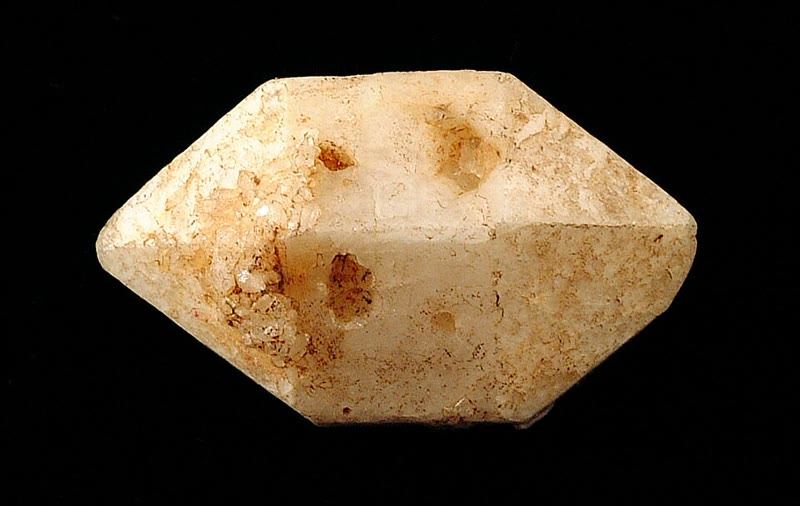
\includegraphics[height=2.75cm]{images/book2/g11-geodil-quartz.jpg}\hfill
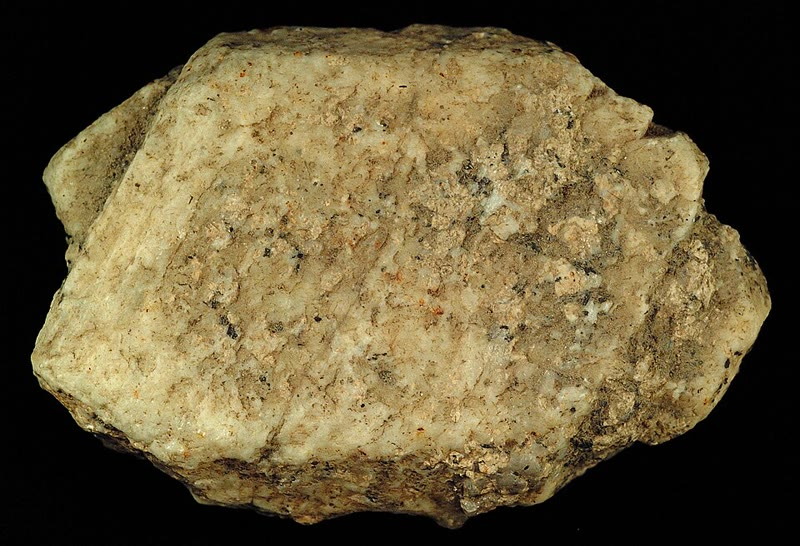
\includegraphics[height=2.75cm]{images/book2/g11-geodil-orthoclase.jpg}\hfill
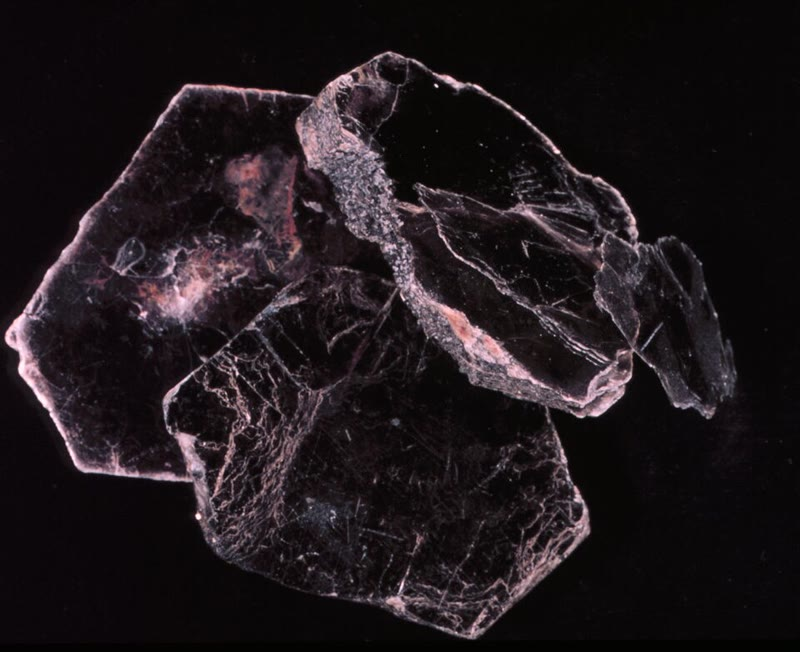
\includegraphics[height=2.75cm]{images/book2/g11-geodil-biotite.jpg}\hfill
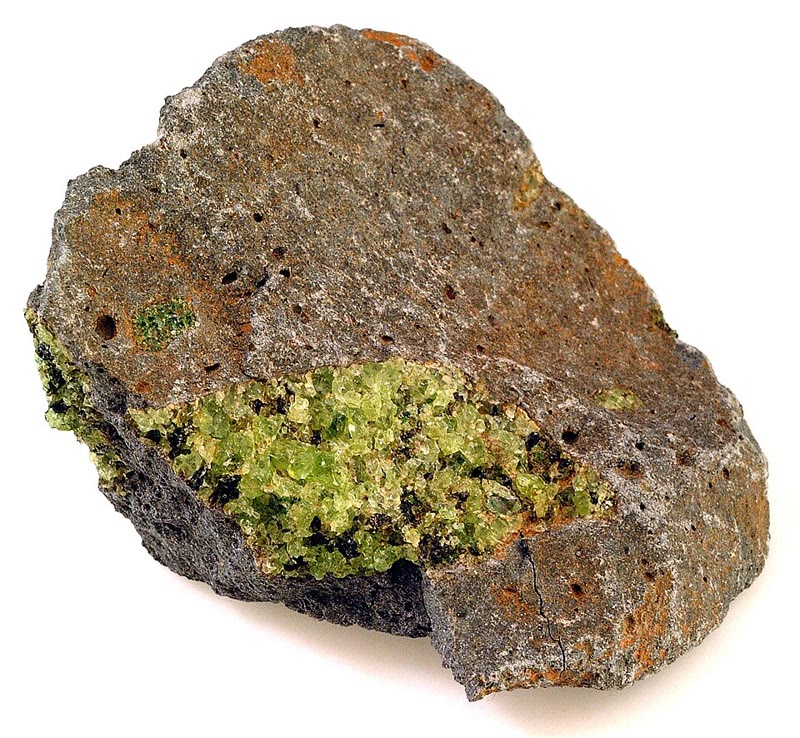
\includegraphics[height=2.75cm]{images/book2/g11-geodil-olivine.jpg}

{\small 四种造岩矿物。自左至右依次为：石英晶体，
两端具尖顶的六方柱，长约 \qty{5}{cm}；正长石，
两个晶体连生，长约 \qty{7}{cm}；
六方形黑云母片，长约 \qty{6}{cm}，沿其唯一的\omterm{def:g11:minerals:cleavage}{解理}
裂成\omterm{def:g11:minerals:thin-section}{薄片}；玄武岩中绿色的橄榄石颗粒。
照片：Shannon Heinle, Darla Sondrol, Dexter Perkins 和 Nessa Eull,
Geology Digital Image Library（CC0）。}
\end{omfigure}
% ledger: photo:g11-quartz, photo:g11-orthoclase, photo:g11-biotite, photo:g11-olivine

\section{硅酸盐}

\paragraph{两种元素构成地壳。}大陆地壳的化学组成
由大量岩石的分析得出，以氧化物的百分含量表示：
约 \qty{60.6}{\percent} \ce{SiO2}，
\qty{15.9}{\percent} \ce{Al2O3}等。由这些数据并结合原子质量，
即可求出各元素的质量。氧占大陆地壳质量的 \qty{46}{\percent}，
硅占 \qty{28}{\percent}：两种元素共
约占质量的四分之三。加上六种金属——铝、
铁、钙、镁、钠和钾——它们共占
\qty{99}{\percent} 以上。
% ledger: rg14:crust, ciaaw:O, ciaaw:Si, ciaaw:Al, ciaaw:Fe, ciaaw:Ca, ciaaw:Mg, ciaaw:Na, ciaaw:K, ciaaw:Ti, ciaaw:Mn, ciaaw:P
% values (mineral_density.py): bulk_O 46.36, bulk_Si 28.30, O+Si 74.66, eight elements 99.43

\begin{omfigure}
\begin{tikzpicture}
\begin{axis}[omrecord, width=0.82\linewidth, height=5.6cm, ybar, bar width=14pt,
  ymin=0, ymax=55, xtick=data, enlarge x limits=0.06,
  xticklabels={{O},{Si},{Al},{Fe},{Ca},{Mg},{Na},{K},{Ti},{Mn},{P}},
  ylabel={质量份额（\unit{\percent}）},
  nodes near coords, every node near coord/.append style={font=\scriptsize, /pgf/number format/.cd, fixed, precision=1},
  xmajorgrids=false]
% computed in figdata/grade-11/mineral_density.py; ledger: rg14:crust, ciaaw:*
\addplot[fill=omDef!55, draw=omDef] table[x expr=\coordindex, y=frac] {figdata/out/grade-11-mineral_density-elements.dat};
\end{axis}
\end{tikzpicture}

{\small 大陆地壳的各元素，以占其质量的份额表示，
由其氧化物形式的平均组成计算得出（Rudnick 和 Gao, 2014）。
仅氧和硅就约占质量的四分之三。}
\end{omfigure}

\paragraph{\omterm{def:g11:minerals:silicate}{硅氧四面体}。}硅原子很小，
四个氧原子围绕其排列，位于一个四面体的顶点上，四面体
是一个带四个三角形面的棱锥。该基团含有一个硅离子 \ce{Si^4+} 和
四个氧离子 \ce{O^2-}，总电荷为 $4 - 4 \times 2 = -4$，
这一电荷须由其他离子——或其他四面体——来平衡。

\begin{definition}[硅酸盐；硅氧四面体]\label{def:g11:minerals:silicate}
称\emph{硅氧四面体}\index{硅氧四面体}为
由一个硅原子与其周围四个氧原子构成的基团 \ce{SiO4}，
这些氧原子位于四面体的顶点上。称
\emph{硅酸盐}\index{硅酸盐}为由硅氧四面体构成的矿物，
单独存在或通过共享顶点相互连接。
\end{definition}
% ledger: tulane:silicates

四面体通过共享氧原子相连：一个四面体的顶点
即为下一个四面体的顶点。每个四面体共享的顶点数
决定\omterm{def:g11:minerals:silicate}{硅酸盐}的结构及其化学式。
\begin{itemize}
  \item \emph{孤立四面体}，不共享顶点，靠
        其间的金属离子维系在一起：橄榄石，\ce{(Mg,Fe)2SiO4}。
  \item \emph{单链}，每个四面体与相邻四面体共享两个顶点：
        辉石。
  \item \emph{双链}，两条单链并排相连，四面体
        交替共享两个或三个顶点：角闪石。
  \item \emph{层状}，每个四面体共享三个顶点：云母，
        以及土壤中的\omterm{def:g10:soil-formation:clay}{黏土矿物}（见\cref{ch:g10:soil-formation}）。
  \item \emph{架状}，每个四面体共享全部四个顶点，
        并在空间三个方向上延伸：石英，\ce{SiO2}，以及——以铝
        替代部分硅所形成的——长石。
\end{itemize}
% ledger: tulane:silicates

\begin{omfigure}
\begin{tikzpicture}[font=\footnotesize]
  % coordinates generated once by a small script (scratch, not kept): kagome net of side 0.62 cm,
  % a regular tetrahedron in perspective, and a framework piece of five tetrahedra (painter's order)
  % (a) one SiO4 tetrahedron, drawn in perspective; the silicon (black) at its centre
  \fill[omDef!12] (2.300,2.979) -- (1.927,1.372) -- (1.221,0.629) -- (3.752,0.820) -- cycle;
  \draw[densely dashed, omDef!60, line width=0.6pt] (2.300,2.979) -- (1.927,1.372);
  \draw[omDef!70!black, line width=0.6pt] (2.300,2.979) -- (1.221,0.629);
  \draw[omDef!70!black, line width=0.6pt] (2.300,2.979) -- (3.752,0.820);
  \draw[densely dashed, omDef!60, line width=0.6pt] (1.927,1.372) -- (1.221,0.629);
  \draw[densely dashed, omDef!60, line width=0.6pt] (1.927,1.372) -- (3.752,0.820);
  \draw[omDef!70!black, line width=0.6pt] (1.221,0.629) -- (3.752,0.820);
  \draw[black!55, line width=0.4pt] (2.300,1.450) -- (2.300,2.979);
  \draw[black!55, line width=0.4pt] (2.300,1.450) -- (1.927,1.372);
  \draw[black!55, line width=0.4pt] (2.300,1.450) -- (1.221,0.629);
  \draw[black!55, line width=0.4pt] (2.300,1.450) -- (3.752,0.820);
  \fill[black] (2.300,1.450) circle (2.2pt);
  \filldraw[fill=omThm!35, draw=omThm!80!black, line width=0.4pt] (2.300,2.979) circle (4.2pt);
  \filldraw[fill=omThm!35, draw=omThm!80!black, line width=0.4pt] (1.927,1.372) circle (4.2pt);
  \filldraw[fill=omThm!35, draw=omThm!80!black, line width=0.4pt] (1.221,0.629) circle (4.2pt);
  \filldraw[fill=omThm!35, draw=omThm!80!black, line width=0.4pt] (3.752,0.820) circle (4.2pt);
  % coordinates for labels: Si 2.300,1.450; apex 2.300,2.979
  % (b) isolated tetrahedra (olivine)
  \filldraw[fill=omDef!22, draw=omDef!70!black, line width=0.5pt] (6.200,0.900) -- (6.820,0.900) -- (6.510,1.437) -- cycle;
  \fill[black] (6.510,1.079) circle (0.9pt);
  \filldraw[fill=omDef!22, draw=omDef!70!black, line width=0.5pt] (8.370,1.437) -- (8.990,1.437) -- (8.680,1.974) -- cycle;
  \fill[black] (8.680,1.616) circle (0.9pt);
  \filldraw[fill=omDef!22, draw=omDef!70!black, line width=0.5pt] (8.060,1.974) -- (7.750,2.511) -- (8.370,2.511) -- cycle;
  \fill[black] (8.060,2.332) circle (0.9pt);
  \filldraw[fill=omDef!22, draw=omDef!70!black, line width=0.5pt] (8.990,0.363) -- (9.610,0.363) -- (9.300,0.900) -- cycle;
  \fill[black] (9.300,0.542) circle (0.9pt);
  \filldraw[fill=omDef!22, draw=omDef!70!black, line width=0.5pt] (9.920,1.974) -- (9.610,2.511) -- (10.230,2.511) -- cycle;
  \fill[black] (9.920,2.332) circle (0.9pt);
  \filldraw[fill=omThm!35, draw=omThm!80!black, line width=0.4pt] (6.200,0.900) circle (1.9pt);
  \filldraw[fill=omThm!35, draw=omThm!80!black, line width=0.4pt] (6.510,1.437) circle (1.9pt);
  \filldraw[fill=omThm!35, draw=omThm!80!black, line width=0.4pt] (6.820,0.900) circle (1.9pt);
  \filldraw[fill=omThm!35, draw=omThm!80!black, line width=0.4pt] (7.750,2.511) circle (1.9pt);
  \filldraw[fill=omThm!35, draw=omThm!80!black, line width=0.4pt] (8.060,1.974) circle (1.9pt);
  \filldraw[fill=omThm!35, draw=omThm!80!black, line width=0.4pt] (8.370,2.511) circle (1.9pt);
  \filldraw[fill=omThm!35, draw=omThm!80!black, line width=0.4pt] (8.370,1.437) circle (1.9pt);
  \filldraw[fill=omThm!35, draw=omThm!80!black, line width=0.4pt] (8.680,1.974) circle (1.9pt);
  \filldraw[fill=omThm!35, draw=omThm!80!black, line width=0.4pt] (8.990,1.437) circle (1.9pt);
  \filldraw[fill=omThm!35, draw=omThm!80!black, line width=0.4pt] (9.610,2.511) circle (1.9pt);
  \filldraw[fill=omThm!35, draw=omThm!80!black, line width=0.4pt] (8.990,0.363) circle (1.9pt);
  \filldraw[fill=omThm!35, draw=omThm!80!black, line width=0.4pt] (9.300,0.900) circle (1.9pt);
  \filldraw[fill=omThm!35, draw=omThm!80!black, line width=0.4pt] (9.920,1.974) circle (1.9pt);
  \filldraw[fill=omThm!35, draw=omThm!80!black, line width=0.4pt] (10.230,2.511) circle (1.9pt);
  \filldraw[fill=omThm!35, draw=omThm!80!black, line width=0.4pt] (9.610,0.363) circle (1.9pt);
  % (c) single chain (pyroxenes)
  \filldraw[fill=omDef!22, draw=omDef!70!black, line width=0.5pt] (11.400,1.600) -- (12.020,1.600) -- (11.710,2.137) -- cycle;
  \fill[black] (11.710,1.779) circle (0.9pt);
  \filldraw[fill=omDef!22, draw=omDef!70!black, line width=0.5pt] (12.330,1.063) -- (12.020,1.600) -- (12.640,1.600) -- cycle;
  \fill[black] (12.330,1.421) circle (0.9pt);
  \filldraw[fill=omDef!22, draw=omDef!70!black, line width=0.5pt] (12.640,1.600) -- (13.260,1.600) -- (12.950,2.137) -- cycle;
  \fill[black] (12.950,1.779) circle (0.9pt);
  \filldraw[fill=omDef!22, draw=omDef!70!black, line width=0.5pt] (13.570,1.063) -- (13.260,1.600) -- (13.880,1.600) -- cycle;
  \fill[black] (13.570,1.421) circle (0.9pt);
  \filldraw[fill=omDef!22, draw=omDef!70!black, line width=0.5pt] (13.880,1.600) -- (14.500,1.600) -- (14.190,2.137) -- cycle;
  \fill[black] (14.190,1.779) circle (0.9pt);
  \filldraw[fill=omDef!22, draw=omDef!70!black, line width=0.5pt] (14.810,1.063) -- (14.500,1.600) -- (15.120,1.600) -- cycle;
  \fill[black] (14.810,1.421) circle (0.9pt);
  \filldraw[fill=omDef!22, draw=omDef!70!black, line width=0.5pt] (15.120,1.600) -- (15.740,1.600) -- (15.430,2.137) -- cycle;
  \fill[black] (15.430,1.779) circle (0.9pt);
  \filldraw[fill=omThm!35, draw=omThm!80!black, line width=0.4pt] (11.400,1.600) circle (1.9pt);
  \filldraw[fill=omThm!35, draw=omThm!80!black, line width=0.4pt] (11.710,2.137) circle (1.9pt);
  \filldraw[fill=omThm!35, draw=omThm!80!black, line width=0.4pt] (12.020,1.600) circle (1.9pt);
  \filldraw[fill=omThm!35, draw=omThm!80!black, line width=0.4pt] (12.330,1.063) circle (1.9pt);
  \filldraw[fill=omThm!35, draw=omThm!80!black, line width=0.4pt] (12.640,1.600) circle (1.9pt);
  \filldraw[fill=omThm!35, draw=omThm!80!black, line width=0.4pt] (12.950,2.137) circle (1.9pt);
  \filldraw[fill=omThm!35, draw=omThm!80!black, line width=0.4pt] (13.260,1.600) circle (1.9pt);
  \filldraw[fill=omThm!35, draw=omThm!80!black, line width=0.4pt] (13.570,1.063) circle (1.9pt);
  \filldraw[fill=omThm!35, draw=omThm!80!black, line width=0.4pt] (13.880,1.600) circle (1.9pt);
  \filldraw[fill=omThm!35, draw=omThm!80!black, line width=0.4pt] (14.190,2.137) circle (1.9pt);
  \filldraw[fill=omThm!35, draw=omThm!80!black, line width=0.4pt] (14.500,1.600) circle (1.9pt);
  \filldraw[fill=omThm!35, draw=omThm!80!black, line width=0.4pt] (14.810,1.063) circle (1.9pt);
  \filldraw[fill=omThm!35, draw=omThm!80!black, line width=0.4pt] (15.120,1.600) circle (1.9pt);
  \filldraw[fill=omThm!35, draw=omThm!80!black, line width=0.4pt] (15.430,2.137) circle (1.9pt);
  \filldraw[fill=omThm!35, draw=omThm!80!black, line width=0.4pt] (15.740,1.600) circle (1.9pt);
  % (d) double chain (amphiboles)
  \filldraw[fill=omDef!22, draw=omDef!70!black, line width=0.5pt] (0.600,-3.550) -- (1.220,-3.550) -- (0.910,-3.013) -- cycle;
  \fill[black] (0.910,-3.371) circle (0.9pt);
  \filldraw[fill=omDef!22, draw=omDef!70!black, line width=0.5pt] (1.530,-4.087) -- (1.220,-3.550) -- (1.840,-3.550) -- cycle;
  \fill[black] (1.530,-3.729) circle (0.9pt);
  \filldraw[fill=omDef!22, draw=omDef!70!black, line width=0.5pt] (1.840,-3.550) -- (2.460,-3.550) -- (2.150,-3.013) -- cycle;
  \fill[black] (2.150,-3.371) circle (0.9pt);
  \filldraw[fill=omDef!22, draw=omDef!70!black, line width=0.5pt] (2.770,-4.087) -- (2.460,-3.550) -- (3.080,-3.550) -- cycle;
  \fill[black] (2.770,-3.729) circle (0.9pt);
  \filldraw[fill=omDef!22, draw=omDef!70!black, line width=0.5pt] (3.080,-3.550) -- (3.700,-3.550) -- (3.390,-3.013) -- cycle;
  \fill[black] (3.390,-3.371) circle (0.9pt);
  \filldraw[fill=omDef!22, draw=omDef!70!black, line width=0.5pt] (4.010,-4.087) -- (3.700,-3.550) -- (4.320,-3.550) -- cycle;
  \fill[black] (4.010,-3.729) circle (0.9pt);
  \filldraw[fill=omDef!22, draw=omDef!70!black, line width=0.5pt] (4.320,-3.550) -- (4.940,-3.550) -- (4.630,-3.013) -- cycle;
  \fill[black] (4.630,-3.371) circle (0.9pt);
  \filldraw[fill=omDef!22, draw=omDef!70!black, line width=0.5pt] (0.910,-3.013) -- (0.600,-2.476) -- (1.220,-2.476) -- cycle;
  \fill[black] (0.910,-2.655) circle (0.9pt);
  \filldraw[fill=omDef!22, draw=omDef!70!black, line width=0.5pt] (1.220,-2.476) -- (1.840,-2.476) -- (1.530,-1.939) -- cycle;
  \fill[black] (1.530,-2.297) circle (0.9pt);
  \filldraw[fill=omDef!22, draw=omDef!70!black, line width=0.5pt] (2.150,-3.013) -- (1.840,-2.476) -- (2.460,-2.476) -- cycle;
  \fill[black] (2.150,-2.655) circle (0.9pt);
  \filldraw[fill=omDef!22, draw=omDef!70!black, line width=0.5pt] (2.460,-2.476) -- (3.080,-2.476) -- (2.770,-1.939) -- cycle;
  \fill[black] (2.770,-2.297) circle (0.9pt);
  \filldraw[fill=omDef!22, draw=omDef!70!black, line width=0.5pt] (3.390,-3.013) -- (3.080,-2.476) -- (3.700,-2.476) -- cycle;
  \fill[black] (3.390,-2.655) circle (0.9pt);
  \filldraw[fill=omDef!22, draw=omDef!70!black, line width=0.5pt] (3.700,-2.476) -- (4.320,-2.476) -- (4.010,-1.939) -- cycle;
  \fill[black] (4.010,-2.297) circle (0.9pt);
  \filldraw[fill=omDef!22, draw=omDef!70!black, line width=0.5pt] (4.630,-3.013) -- (4.320,-2.476) -- (4.940,-2.476) -- cycle;
  \fill[black] (4.630,-2.655) circle (0.9pt);
  \filldraw[fill=omThm!35, draw=omThm!80!black, line width=0.4pt] (0.600,-2.476) circle (1.9pt);
  \filldraw[fill=omThm!35, draw=omThm!80!black, line width=0.4pt] (0.600,-3.550) circle (1.9pt);
  \filldraw[fill=omThm!35, draw=omThm!80!black, line width=0.4pt] (0.910,-3.013) circle (1.9pt);
  \filldraw[fill=omThm!35, draw=omThm!80!black, line width=0.4pt] (1.220,-2.476) circle (1.9pt);
  \filldraw[fill=omThm!35, draw=omThm!80!black, line width=0.4pt] (1.530,-1.939) circle (1.9pt);
  \filldraw[fill=omThm!35, draw=omThm!80!black, line width=0.4pt] (1.220,-3.550) circle (1.9pt);
  \filldraw[fill=omThm!35, draw=omThm!80!black, line width=0.4pt] (1.840,-2.476) circle (1.9pt);
  \filldraw[fill=omThm!35, draw=omThm!80!black, line width=0.4pt] (1.530,-4.087) circle (1.9pt);
  \filldraw[fill=omThm!35, draw=omThm!80!black, line width=0.4pt] (1.840,-3.550) circle (1.9pt);
  \filldraw[fill=omThm!35, draw=omThm!80!black, line width=0.4pt] (2.150,-3.013) circle (1.9pt);
  \filldraw[fill=omThm!35, draw=omThm!80!black, line width=0.4pt] (2.460,-2.476) circle (1.9pt);
  \filldraw[fill=omThm!35, draw=omThm!80!black, line width=0.4pt] (2.770,-1.939) circle (1.9pt);
  \filldraw[fill=omThm!35, draw=omThm!80!black, line width=0.4pt] (2.460,-3.550) circle (1.9pt);
  \filldraw[fill=omThm!35, draw=omThm!80!black, line width=0.4pt] (3.080,-2.476) circle (1.9pt);
  \filldraw[fill=omThm!35, draw=omThm!80!black, line width=0.4pt] (2.770,-4.087) circle (1.9pt);
  \filldraw[fill=omThm!35, draw=omThm!80!black, line width=0.4pt] (3.080,-3.550) circle (1.9pt);
  \filldraw[fill=omThm!35, draw=omThm!80!black, line width=0.4pt] (3.390,-3.013) circle (1.9pt);
  \filldraw[fill=omThm!35, draw=omThm!80!black, line width=0.4pt] (3.700,-2.476) circle (1.9pt);
  \filldraw[fill=omThm!35, draw=omThm!80!black, line width=0.4pt] (4.010,-1.939) circle (1.9pt);
  \filldraw[fill=omThm!35, draw=omThm!80!black, line width=0.4pt] (3.700,-3.550) circle (1.9pt);
  \filldraw[fill=omThm!35, draw=omThm!80!black, line width=0.4pt] (4.320,-2.476) circle (1.9pt);
  \filldraw[fill=omThm!35, draw=omThm!80!black, line width=0.4pt] (4.010,-4.087) circle (1.9pt);
  \filldraw[fill=omThm!35, draw=omThm!80!black, line width=0.4pt] (4.320,-3.550) circle (1.9pt);
  \filldraw[fill=omThm!35, draw=omThm!80!black, line width=0.4pt] (4.630,-3.013) circle (1.9pt);
  \filldraw[fill=omThm!35, draw=omThm!80!black, line width=0.4pt] (4.940,-2.476) circle (1.9pt);
  \filldraw[fill=omThm!35, draw=omThm!80!black, line width=0.4pt] (4.940,-3.550) circle (1.9pt);
  % (e) sheet (micas)
  \filldraw[fill=omDef!22, draw=omDef!70!black, line width=0.5pt] (5.900,-4.100) -- (6.520,-4.100) -- (6.210,-3.563) -- cycle;
  \fill[black] (6.210,-3.921) circle (0.9pt);
  \filldraw[fill=omDef!22, draw=omDef!70!black, line width=0.5pt] (7.140,-4.100) -- (7.760,-4.100) -- (7.450,-3.563) -- cycle;
  \fill[black] (7.450,-3.921) circle (0.9pt);
  \filldraw[fill=omDef!22, draw=omDef!70!black, line width=0.5pt] (8.380,-4.100) -- (9.000,-4.100) -- (8.690,-3.563) -- cycle;
  \fill[black] (8.690,-3.921) circle (0.9pt);
  \filldraw[fill=omDef!22, draw=omDef!70!black, line width=0.5pt] (9.620,-4.100) -- (10.240,-4.100) -- (9.930,-3.563) -- cycle;
  \fill[black] (9.930,-3.921) circle (0.9pt);
  \filldraw[fill=omDef!22, draw=omDef!70!black, line width=0.5pt] (6.210,-3.563) -- (5.900,-3.026) -- (6.520,-3.026) -- cycle;
  \fill[black] (6.210,-3.205) circle (0.9pt);
  \filldraw[fill=omDef!22, draw=omDef!70!black, line width=0.5pt] (7.450,-3.563) -- (7.140,-3.026) -- (7.760,-3.026) -- cycle;
  \fill[black] (7.450,-3.205) circle (0.9pt);
  \filldraw[fill=omDef!22, draw=omDef!70!black, line width=0.5pt] (8.690,-3.563) -- (8.380,-3.026) -- (9.000,-3.026) -- cycle;
  \fill[black] (8.690,-3.205) circle (0.9pt);
  \filldraw[fill=omDef!22, draw=omDef!70!black, line width=0.5pt] (9.930,-3.563) -- (9.620,-3.026) -- (10.240,-3.026) -- cycle;
  \fill[black] (9.930,-3.205) circle (0.9pt);
  \filldraw[fill=omDef!22, draw=omDef!70!black, line width=0.5pt] (6.520,-3.026) -- (7.140,-3.026) -- (6.830,-2.489) -- cycle;
  \fill[black] (6.830,-2.847) circle (0.9pt);
  \filldraw[fill=omDef!22, draw=omDef!70!black, line width=0.5pt] (7.760,-3.026) -- (8.380,-3.026) -- (8.070,-2.489) -- cycle;
  \fill[black] (8.070,-2.847) circle (0.9pt);
  \filldraw[fill=omDef!22, draw=omDef!70!black, line width=0.5pt] (9.000,-3.026) -- (9.620,-3.026) -- (9.310,-2.489) -- cycle;
  \fill[black] (9.310,-2.847) circle (0.9pt);
  \filldraw[fill=omDef!22, draw=omDef!70!black, line width=0.5pt] (6.830,-2.489) -- (6.520,-1.952) -- (7.140,-1.952) -- cycle;
  \fill[black] (6.830,-2.131) circle (0.9pt);
  \filldraw[fill=omDef!22, draw=omDef!70!black, line width=0.5pt] (8.070,-2.489) -- (7.760,-1.952) -- (8.380,-1.952) -- cycle;
  \fill[black] (8.070,-2.131) circle (0.9pt);
  \filldraw[fill=omDef!22, draw=omDef!70!black, line width=0.5pt] (9.310,-2.489) -- (9.000,-1.952) -- (9.620,-1.952) -- cycle;
  \fill[black] (9.310,-2.131) circle (0.9pt);
  \filldraw[fill=omDef!22, draw=omDef!70!black, line width=0.5pt] (5.900,-1.952) -- (6.520,-1.952) -- (6.210,-1.415) -- cycle;
  \fill[black] (6.210,-1.773) circle (0.9pt);
  \filldraw[fill=omDef!22, draw=omDef!70!black, line width=0.5pt] (7.140,-1.952) -- (7.760,-1.952) -- (7.450,-1.415) -- cycle;
  \fill[black] (7.450,-1.773) circle (0.9pt);
  \filldraw[fill=omDef!22, draw=omDef!70!black, line width=0.5pt] (8.380,-1.952) -- (9.000,-1.952) -- (8.690,-1.415) -- cycle;
  \fill[black] (8.690,-1.773) circle (0.9pt);
  \filldraw[fill=omDef!22, draw=omDef!70!black, line width=0.5pt] (9.620,-1.952) -- (10.240,-1.952) -- (9.930,-1.415) -- cycle;
  \fill[black] (9.930,-1.773) circle (0.9pt);
  \filldraw[fill=omThm!35, draw=omThm!80!black, line width=0.4pt] (5.900,-1.952) circle (1.9pt);
  \filldraw[fill=omThm!35, draw=omThm!80!black, line width=0.4pt] (6.210,-1.415) circle (1.9pt);
  \filldraw[fill=omThm!35, draw=omThm!80!black, line width=0.4pt] (5.900,-3.026) circle (1.9pt);
  \filldraw[fill=omThm!35, draw=omThm!80!black, line width=0.4pt] (6.520,-1.952) circle (1.9pt);
  \filldraw[fill=omThm!35, draw=omThm!80!black, line width=0.4pt] (5.900,-4.100) circle (1.9pt);
  \filldraw[fill=omThm!35, draw=omThm!80!black, line width=0.4pt] (6.210,-3.563) circle (1.9pt);
  \filldraw[fill=omThm!35, draw=omThm!80!black, line width=0.4pt] (6.520,-3.026) circle (1.9pt);
  \filldraw[fill=omThm!35, draw=omThm!80!black, line width=0.4pt] (6.830,-2.489) circle (1.9pt);
  \filldraw[fill=omThm!35, draw=omThm!80!black, line width=0.4pt] (7.140,-1.952) circle (1.9pt);
  \filldraw[fill=omThm!35, draw=omThm!80!black, line width=0.4pt] (7.450,-1.415) circle (1.9pt);
  \filldraw[fill=omThm!35, draw=omThm!80!black, line width=0.4pt] (6.520,-4.100) circle (1.9pt);
  \filldraw[fill=omThm!35, draw=omThm!80!black, line width=0.4pt] (7.140,-3.026) circle (1.9pt);
  \filldraw[fill=omThm!35, draw=omThm!80!black, line width=0.4pt] (7.760,-1.952) circle (1.9pt);
  \filldraw[fill=omThm!35, draw=omThm!80!black, line width=0.4pt] (7.140,-4.100) circle (1.9pt);
  \filldraw[fill=omThm!35, draw=omThm!80!black, line width=0.4pt] (7.450,-3.563) circle (1.9pt);
  \filldraw[fill=omThm!35, draw=omThm!80!black, line width=0.4pt] (7.760,-3.026) circle (1.9pt);
  \filldraw[fill=omThm!35, draw=omThm!80!black, line width=0.4pt] (8.070,-2.489) circle (1.9pt);
  \filldraw[fill=omThm!35, draw=omThm!80!black, line width=0.4pt] (8.380,-1.952) circle (1.9pt);
  \filldraw[fill=omThm!35, draw=omThm!80!black, line width=0.4pt] (8.690,-1.415) circle (1.9pt);
  \filldraw[fill=omThm!35, draw=omThm!80!black, line width=0.4pt] (7.760,-4.100) circle (1.9pt);
  \filldraw[fill=omThm!35, draw=omThm!80!black, line width=0.4pt] (8.380,-3.026) circle (1.9pt);
  \filldraw[fill=omThm!35, draw=omThm!80!black, line width=0.4pt] (9.000,-1.952) circle (1.9pt);
  \filldraw[fill=omThm!35, draw=omThm!80!black, line width=0.4pt] (8.380,-4.100) circle (1.9pt);
  \filldraw[fill=omThm!35, draw=omThm!80!black, line width=0.4pt] (8.690,-3.563) circle (1.9pt);
  \filldraw[fill=omThm!35, draw=omThm!80!black, line width=0.4pt] (9.000,-3.026) circle (1.9pt);
  \filldraw[fill=omThm!35, draw=omThm!80!black, line width=0.4pt] (9.310,-2.489) circle (1.9pt);
  \filldraw[fill=omThm!35, draw=omThm!80!black, line width=0.4pt] (9.620,-1.952) circle (1.9pt);
  \filldraw[fill=omThm!35, draw=omThm!80!black, line width=0.4pt] (9.930,-1.415) circle (1.9pt);
  \filldraw[fill=omThm!35, draw=omThm!80!black, line width=0.4pt] (9.000,-4.100) circle (1.9pt);
  \filldraw[fill=omThm!35, draw=omThm!80!black, line width=0.4pt] (9.620,-3.026) circle (1.9pt);
  \filldraw[fill=omThm!35, draw=omThm!80!black, line width=0.4pt] (10.240,-1.952) circle (1.9pt);
  \filldraw[fill=omThm!35, draw=omThm!80!black, line width=0.4pt] (9.620,-4.100) circle (1.9pt);
  \filldraw[fill=omThm!35, draw=omThm!80!black, line width=0.4pt] (9.930,-3.563) circle (1.9pt);
  \filldraw[fill=omThm!35, draw=omThm!80!black, line width=0.4pt] (10.240,-3.026) circle (1.9pt);
  \filldraw[fill=omThm!35, draw=omThm!80!black, line width=0.4pt] (10.240,-4.100) circle (1.9pt);
  % (f) framework: a tetrahedron sharing all four corners
  \filldraw[fill=omThm!35, draw=omThm!80!black, line width=0.4pt] (12.990,-1.963) circle (2.1pt);
  \filldraw[fill=omThm!35, draw=omThm!80!black, line width=0.4pt] (12.896,-3.062) circle (2.1pt);
  \filldraw[fill=omDef!14, draw=omDef!70!black, line width=0.45pt, fill opacity=0.85] (12.896,-3.062) -- (12.990,-1.963) -- (12.299,-2.380) -- cycle;
  \filldraw[fill=omThm!35, draw=omThm!80!black, line width=0.4pt] (15.186,-2.119) circle (2.1pt);
  \filldraw[fill=omDef!14, draw=omDef!70!black, line width=0.45pt, fill opacity=0.85] (12.896,-3.062) -- (13.398,-2.458) -- (12.990,-1.963) -- cycle;
  \filldraw[fill=omThm!35, draw=omThm!80!black, line width=0.4pt] (15.092,-3.219) circle (2.1pt);
  \fill[black] (12.896,-2.466) circle (1.1pt);
  \filldraw[fill=omDef!34, draw=omDef!70!black, line width=0.45pt, fill opacity=0.85] (13.398,-2.458) -- (12.990,-1.963) -- (12.299,-2.380) -- cycle;
  \filldraw[fill=omDef!14, draw=omDef!70!black, line width=0.45pt, fill opacity=0.85] (15.092,-3.219) -- (15.186,-2.119) -- (14.496,-2.536) -- cycle;
  \filldraw[fill=omDef!25, draw=omDef!70!black, line width=0.45pt, fill opacity=0.85] (12.896,-3.062) -- (12.299,-2.380) -- (13.398,-2.458) -- cycle;
  \filldraw[fill=omDef!14, draw=omDef!70!black, line width=0.45pt, fill opacity=0.85] (15.092,-3.219) -- (15.595,-2.614) -- (15.186,-2.119) -- cycle;
  \fill[black] (15.092,-2.622) circle (1.1pt);
  \filldraw[fill=omThm!35, draw=omThm!80!black, line width=0.4pt] (12.299,-2.380) circle (2.1pt);
  \filldraw[fill=omDef!34, draw=omDef!70!black, line width=0.45pt, fill opacity=0.85] (15.595,-2.614) -- (15.186,-2.119) -- (14.496,-2.536) -- cycle;
  \filldraw[fill=omDef!25, draw=omDef!70!black, line width=0.45pt, fill opacity=0.85] (15.092,-3.219) -- (14.496,-2.536) -- (15.595,-2.614) -- cycle;
  \filldraw[fill=omThm!35, draw=omThm!80!black, line width=0.4pt] (13.398,-2.458) circle (2.1pt);
  \filldraw[fill=omThm!35, draw=omThm!80!black, line width=0.4pt] (14.496,-2.536) circle (2.1pt);
  \filldraw[fill=omDef!14, draw=omDef!70!black, line width=0.45pt, fill opacity=0.85] (13.900,-1.853) -- (14.496,-2.536) -- (13.398,-2.458) -- cycle;
  \filldraw[fill=omThm!35, draw=omThm!80!black, line width=0.4pt] (15.595,-2.614) circle (2.1pt);
  \filldraw[fill=omDef!14, draw=omDef!70!black, line width=0.45pt, fill opacity=0.85] (13.398,-2.458) -- (13.806,-2.953) -- (14.496,-2.536) -- cycle;
  \fill[black] (13.900,-2.450) circle (1.1pt);
  \filldraw[fill=omDef!22, draw=omDef!70!black, line width=0.45pt, fill opacity=0.85] (13.900,-1.853) -- (13.398,-2.458) -- (13.806,-2.953) -- cycle;
  \filldraw[fill=omDef!37, draw=omDef!70!black, line width=0.45pt, fill opacity=0.85] (13.900,-1.853) -- (13.806,-2.953) -- (14.496,-2.536) -- cycle;
  \filldraw[fill=omThm!35, draw=omThm!80!black, line width=0.4pt] (13.994,-0.754) circle (2.1pt);
  \filldraw[fill=omThm!35, draw=omThm!80!black, line width=0.4pt] (13.900,-1.853) circle (2.1pt);
  \filldraw[fill=omThm!35, draw=omThm!80!black, line width=0.4pt] (13.806,-2.953) circle (2.1pt);
  \filldraw[fill=omDef!14, draw=omDef!70!black, line width=0.45pt, fill opacity=0.85] (13.900,-1.853) -- (13.994,-0.754) -- (13.304,-1.171) -- cycle;
  \filldraw[fill=omDef!14, draw=omDef!70!black, line width=0.45pt, fill opacity=0.85] (13.900,-1.853) -- (14.402,-1.249) -- (13.994,-0.754) -- cycle;
  \filldraw[fill=omThm!35, draw=omThm!80!black, line width=0.4pt] (13.712,-4.053) circle (2.1pt);
  \fill[black] (13.900,-1.256) circle (1.1pt);
  \filldraw[fill=omDef!14, draw=omDef!70!black, line width=0.45pt, fill opacity=0.85] (13.712,-4.053) -- (13.806,-2.953) -- (13.116,-3.370) -- cycle;
  \filldraw[fill=omDef!34, draw=omDef!70!black, line width=0.45pt, fill opacity=0.85] (14.402,-1.249) -- (13.994,-0.754) -- (13.304,-1.171) -- cycle;
  \filldraw[fill=omDef!14, draw=omDef!70!black, line width=0.45pt, fill opacity=0.85] (13.712,-4.053) -- (14.214,-3.448) -- (13.806,-2.953) -- cycle;
  \filldraw[fill=omDef!25, draw=omDef!70!black, line width=0.45pt, fill opacity=0.85] (13.900,-1.853) -- (13.304,-1.171) -- (14.402,-1.249) -- cycle;
  \fill[black] (13.712,-3.456) circle (1.1pt);
  \filldraw[fill=omThm!35, draw=omThm!80!black, line width=0.4pt] (13.304,-1.171) circle (2.1pt);
  \filldraw[fill=omDef!34, draw=omDef!70!black, line width=0.45pt, fill opacity=0.85] (14.214,-3.448) -- (13.806,-2.953) -- (13.116,-3.370) -- cycle;
  \filldraw[fill=omDef!25, draw=omDef!70!black, line width=0.45pt, fill opacity=0.85] (13.712,-4.053) -- (13.116,-3.370) -- (14.214,-3.448) -- cycle;
  \filldraw[fill=omThm!35, draw=omThm!80!black, line width=0.4pt] (14.402,-1.249) circle (2.1pt);
  \filldraw[fill=omThm!35, draw=omThm!80!black, line width=0.4pt] (13.116,-3.370) circle (2.1pt);
  \filldraw[fill=omThm!35, draw=omThm!80!black, line width=0.4pt] (14.214,-3.448) circle (2.1pt);
  % labels
  \draw[black!60] (2.30,2.98) -- (3.35,3.25); \node[anchor=west] at (3.35,3.25) {氧};
  \draw[black!60] (2.30,1.45) -- (3.55,2.15); \node[anchor=west] at (3.55,2.15) {硅};
  \node[align=center] at (2.3,-0.15) {(a) 单个四面体，\ce{SiO4}};
  \node[align=center] at (8.2,-0.15) {(b) 孤立四面体：\\橄榄石};
  \node[align=center] at (13.5,-0.15) {(c) 单链：\\辉石};
  \node[align=center] at (2.75,-4.85) {(d) 双链：\\角闪石};
  \node[align=center] at (8.1,-4.85) {(e) 层状：\\云母};
  \node[align=center] at (13.9,-4.85) {(f) 架状：\\石英、长石};
\end{tikzpicture}

{\small (a) 硅–氧四面体：一个硅原子（黑色）和四个氧原子（粉色）
位于四面体的顶点。(b)--(e) 为从上方看到的四面体，每个呈三角形：
圆圈为其底面的氧原子，圆点为硅原子，位于第四个氧原子之下；
两个三角形在一个顶点相接时，共用该顶点的氧原子。
(f) 在架状结构中，每个顶点都被共用，并向三维空间延伸：
此处为一个四面体及其四个相邻四面体。示意图，未按
比例绘制。}
\end{omfigure}
% ledger: tulane:silicates

\begin{proposition}[氧原子计数]\label{prop:g11:minerals:sharing}
在\omterm{def:g11:minerals:silicate}{硅酸盐}中，若每个四面体与其他四面体共用其 $n$ 个顶点，
则每个硅原子对应 $4 - n/2$ 个氧原子。
孤立四面体给出 \ce{SiO4}，单链给出 \ce{SiO3}，层状给出 \ce{Si2O5}，
架状给出 \ce{SiO2}。
\end{proposition}

\begin{proof}
每个四面体含一个硅原子和四个顶点。未被共用的顶点只属于该四面体，
计为一个氧原子；被共用的顶点属于两个四面体，
各计为半个氧原子。设有 $n$ 个被共用的顶点，则一个四面体拥有
$(4 - n) + n/2 = 4 - n/2$ 个氧原子。
取 $n = 0$、$2$、$3$ 和 $4$，则每个硅原子对应的氧原子数分别为 $4$、$3$、$5/2$ 和 $2$，
即 \ce{SiO4}、\ce{SiO3}、\ce{Si2O5} 与 \ce{SiO2}。
\end{proof}

矿物的化学式印证了这一点。辉石类矿物普通辉石含
\ce{(Si,Al)2O6}，即两个 \ce{SiO3}；黑云母为 \ce{AlSi3O10}，
含四个四面体、十个氧原子，即两个 \ce{Si2O5}；长石中，
四个四面体含八个氧原子，即四个 \ce{SiO2}，与石英完全相同。
不过，电荷并不相同。石英呈电中性：在架状结构中，每个氧原子
都被共用，硅与氧的电荷恰好平衡。在其他结构中，
未被共用的氧原子带有多余的负电荷，须由
金属离子平衡——橄榄石中为镁和铁，正长石中为钾。其中
一个铝离子 \ce{Al^3+} 代替一个硅离子 \ce{Si^4+}，便剩下
一个待平衡的电荷。
% ledger: wm:densities (formulas)

\begin{definition}[造岩硅酸盐]\label{def:g11:minerals:rock-forming}
称\emph{造岩硅酸盐}\index{造岩硅酸盐}为
构成大多数常见火成岩和变质岩的六类\omterm{def:g11:minerals:silicate}{硅酸盐}矿物群：
橄榄石、辉石、角闪石、云母、长石与石英。长石有两类：
\emph{钾长石}，如正长石，以及
\emph{斜长石}，
即一系列含钠和钙的长石。
\end{definition}
% ledger: tulane:silicates, wm:densities

\begin{center}
\small
\renewcommand{\arraystretch}{1.25}
\begin{tabular}{|l|l|l|c|}
\hline
\textbf{矿物组（代表）} & \textbf{结构} & \textbf{化学式} & \textbf{密度} \\
 & & & (\unit{g/cm^3}) \\
\hline
橄榄石 & 孤立四面体 & \ce{(Mg,Fe)2SiO4} & 3.32 \\
辉石（普通辉石） & 单链 & \ce{(Ca,Na)(Mg,Fe,Al,Ti)(Si,Al)2O6} & 3.4 \\
角闪石（普通角闪石） & 双链 & \ce{Ca2[Mg4(Al,Fe)]Si7AlO22(OH)2} & 3.23 \\
云母（黑云母） & 层状 & \ce{K(Mg,Fe)3AlSi3O10(OH,F)2} & 3.09 \\
云母（白云母） & 层状 & \ce{KAl2(Si3Al)O10(OH,F)2} & 2.82 \\
钾长石（正长石） & 架状 & \ce{KAlSi3O8} & 2.56 \\
斜长石（更长石） & 架状 & \ce{(Na,Ca)(Si,Al)4O8} & 2.65 \\
石英 & 架状 & \ce{SiO2} & 2.62 \\
\hline
\end{tabular}

\smallskip
{\footnotesize \omterm{def:g11:minerals:rock-forming}{造岩硅酸盐}。化学式与平均密度引自
webmineral.com；括号内以逗号分隔的两种元素，表示二者均可占据
该位置，即两者可在晶体中互相替代。}
\end{center}
% ledger: wm:densities, tulane:silicates

此表蕴含一条贯穿本书的规律。孤立四面体与链状结构的矿物，
富含铁和镁，是最致密的一类，密度高于 \qty{3.2}{g/cm^3}；
架状结构的矿物由硅、铝、钠、钾和钙组成，是最轻的一类，
密度约为 \qty{2.6}{g/cm^3}。云母居于其间。
橄榄石与辉石构成地幔的\omterm{def:g11:ocean-ridges:peridotite}{橄榄岩}；
长石与石英构成大陆的花岗岩。
轻岩石漂浮在重岩石之上。
% ledger: wm:densities

\section{矿物构成岩石}

描述岩石，首先看其所含矿物及比例。前面各章中遇到过三种岩石，
可体现这一范围：
\begin{itemize}
  \item \emph{花岗岩}：石英、钾长石和斜长石，并含少量
        黑云母或白云母——大陆的岩石；
  \item \emph{玄武岩}与\emph{\omterm{def:g11:ocean-ridges:gabbro}{辉长岩}}：斜长石和辉石，常
        含橄榄石——\omterm{def:g11:ocean-ridges:oceanic-lithosphere}{洋壳}的岩石，前者为细粒，
        后者为粗粒（见\cref{ch:g11:igneous-rocks}）；
  \item \emph{\omterm{def:g11:ocean-ridges:peridotite}{橄榄岩}}：主要为橄榄石，含辉石——地幔的
        岩石。
\end{itemize}
% ledger: nps:granite-minerals, photo:g11-basalt-thin-section, photo:g11-olivine

\begin{omfigure}
\begin{tikzpicture}
\begin{axis}[omrecord, width=0.8\linewidth, height=6.4cm, xbar, bar width=8pt,
  xmin=2.4, xmax=3.5, ymin=-0.7, ymax=8.7, ytick={0,...,8},
  yticklabels={正长石, 石英, 更长石, 拉长石, 白云母, 黑云母, 普通角闪石, 橄榄石, 普通辉石},
  xlabel={密度 (\unit{g/cm^3})}, ymajorgrids=false, clip=false]
% computed in figdata/grade-11/mineral_density.py (density_order); ledger: wm:densities
\addplot[fill=omDef!45, draw=omDef] table[x=rho, y=idx] {figdata/out/grade-11-mineral_density-densities.dat};
\draw[omProp, line width=1pt, dashed] (axis cs:2.6427,-0.7) -- (axis cs:2.6427,8.7) node[above, text height=1.6ex, text depth=0.3ex, font=\scriptsize, text=omProp!80!black] {花岗岩};
\draw[omThm, line width=1pt, dashed] (axis cs:3.0015,-0.7) -- (axis cs:3.0015,8.7) node[above, text height=1.6ex, text depth=0.3ex, font=\scriptsize, text=omThm] {玄武岩};
\draw[black!70, line width=1pt, dashed] (axis cs:3.34,-0.7) -- (axis cs:3.34,8.7) node[above, font=\scriptsize] {橄榄岩};
\end{axis}
\end{tikzpicture}

{\small 九种造岩矿物的平均密度（webmineral.com），
以及本节三个例岩石的密度（虚线，由下面的命题算得）：
一块花岗岩由石英、长石和云母组成，
一块玄武岩由斜长石、辉石和少量橄榄石组成，
一块\omterm{def:g11:ocean-ridges:peridotite}{橄榄岩}由橄榄石和辉石组成。}
\end{omfigure}
% values (mineral_density.py): rho_granite 2.6427, rho_basalt 3.0015, rho_peridotite 3.34

岩石的密度由其所含矿物决定。设想一块
体积为 $V$ 的岩石，其中比例为 $\phi_1$ 的部分由第一种矿物组成，
比例为 $\phi_2$ 的部分由第二种矿物组成，依此类推。

\begin{proposition}[由矿物求岩石的密度]\label{prop:g11:minerals:density}
不含孔隙的岩石，由密度分别为 $\rho_1, \rho_2, \dots,
\rho_k$ 的矿物构成，各矿物占岩石体积的比例分别为 $\phi_1, \phi_2, \dots, \phi_k$，
即 $\phi_1 + \dots + \phi_k = 1$，则其密度为
\[
  \rho = \phi_1 \rho_1 + \phi_2 \rho_2 + \dots + \phi_k \rho_k ,
\]
即各矿物密度以其体积比例为权重的
加权平均。
\end{proposition}

\begin{proof}
在体积为 $V$ 的岩石中，矿物 $i$ 占据体积 $\phi_i V$，
质量为 $\rho_i \phi_i V$。无孔隙时，岩石的质量等于这些质量之和，
$m = (\phi_1 \rho_1 + \dots + \phi_k \rho_k)\,V$，
其密度为 $m/V$。
\end{proof}

体积比例如何测定？可在岩石的平整切面上，或在
\omterm{def:g11:minerals:thin-section}{薄片}上（下一节介绍），布置规则的网格点，在每个点上
记下其下方的矿物。若颗粒无序分布，
落在某矿物上的点所占比例，即估计该矿物
所占面积的比例，也就是其占体积的比例：
\omterm{def:g11:minerals:thin-section}{薄片}可以很好地代表整块岩石。这种方法称为
\emph{点计数}。

\begin{example}[一块富含石英与钾长石的浅色花岗岩]
一次点计数得到石英 \qty{35}{\percent}（\qty{2.62}{g/cm^3}）、
正长石 \qty{50}{\percent}（\qty{2.56}{g/cm^3}）和
更长石 \qty{15}{\percent}（\qty{2.65}{g/cm^3}）。该岩石的密度为
\[
  \rho = 0.35 \times 2.62 + 0.50 \times 2.56 + 0.15 \times 2.65
       = 0.917 + 1.280 + 0.398 \approx \qty{2.59}{g/cm^3}.
\]
实测结果支持这一数量级：在加利福尼亚州内华达山脉，
从约两百个花岗质岩体上称量了 \num{6454} 块岩石样品，
平均值为 \qty{2.69}{g/cm^3}；富含二氧化硅和钾的花岗岩，
如本例，密度均低于 \qty{2.6}{g/cm^3}。
\end{example}
% ledger: wm:densities, usgs91:sierra

\section{薄片}

手持放大镜只能看清直径约一毫米的颗粒。要看清更细的颗粒，并准确地
鉴定它们，地质学家便借助显微镜观察岩石，
——不是观察其表面，而是透过岩石本身观察。

\begin{definition}[薄片；偏光显微镜]\label{def:g11:minerals:thin-section}
\emph{薄片}\index{薄片}是将岩石磨至
\qty{0.03}{mm} 厚并固定在载玻片上的切片：在此厚度下，
光线可穿过大多数矿物。\emph{偏光
显微镜}\index{偏光显微镜}是一种装有两块
偏光滤光片的显微镜，一块在载玻片下方，一块在其上方。
切片在仅用下方滤光片的\emph{单偏光}下观察，
在上方滤光片加上、且其方向与下方滤光片垂直时，
则为\emph{正交偏光}下的观察。
\end{definition}
% ledger: tulane:thin-section

\begin{omfigure}
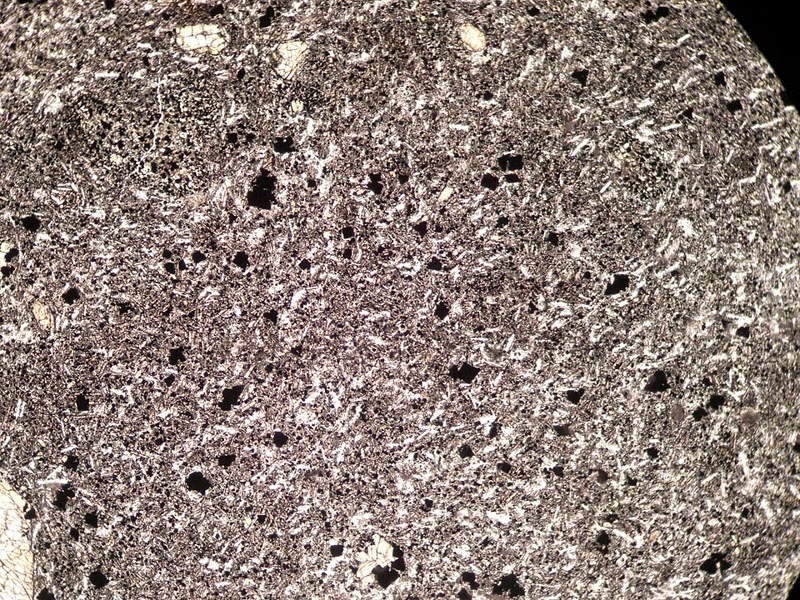
\includegraphics[height=3.6cm]{images/book2/g11-chmee2-basalt-ppl.jpg}\hfill
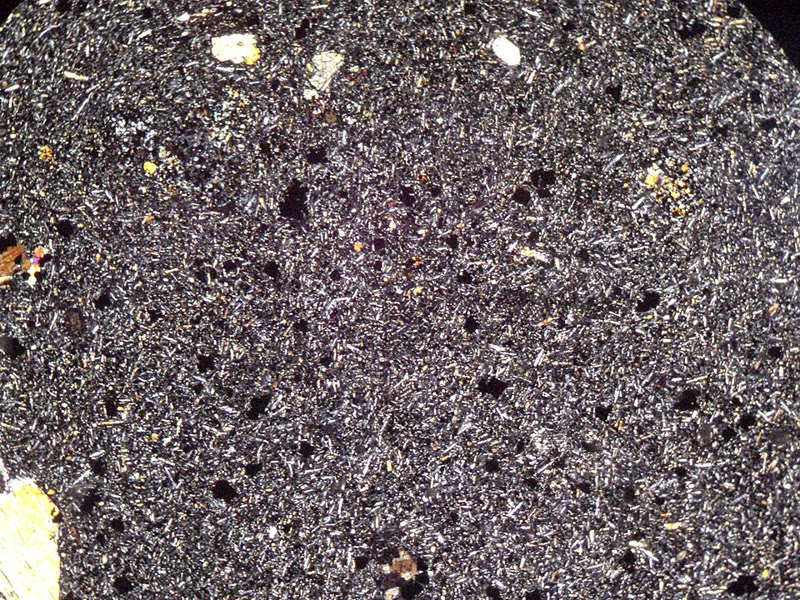
\includegraphics[height=3.6cm]{images/book2/g11-chmee2-basalt-xpl.jpg}\hfill
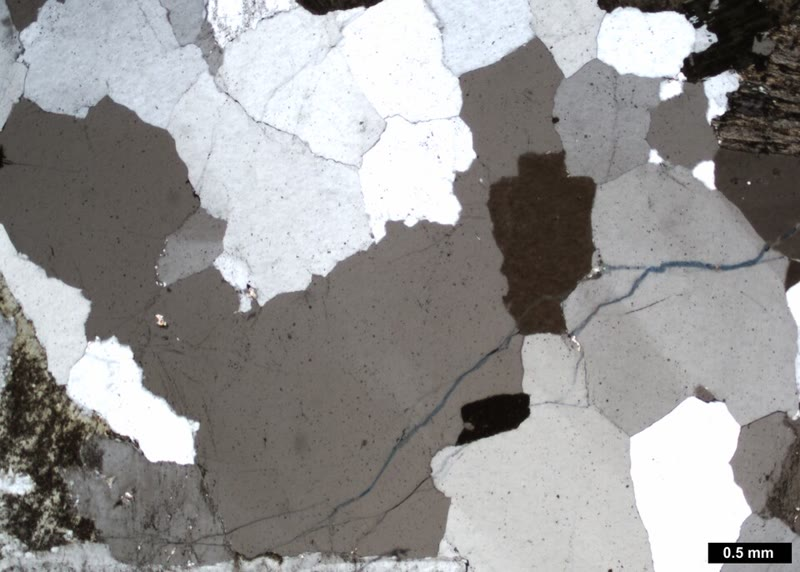
\includegraphics[height=3.6cm]{images/book2/g11-rygel-granite-xpl.jpg}

{\small 左图和中图：同一块玄武岩\omterm{def:g11:minerals:thin-section}{薄片}，分别在单偏光与
正交偏光下拍摄。该岩石为细粒结构：细长的小晶体，
主要为斜长石，还有黑色斑点，两种光下均不透光；
在正交偏光下，晶体呈现灰色和
彩色。照片：
Chmee2（CC~BY-SA~3.0）。右图：花岗岩中的石英晶体，在正交偏光下
呈现各自不同深浅的灰色（比例尺
为 \qty{0.5}{mm}）。照片：Michael C.~Rygel（CC~BY-SA~3.0）。}
\end{omfigure}
% ledger: photo:g11-basalt-thin-section, photo:g11-granite-thin-section

在单偏光下，\omterm{def:g11:minerals:thin-section}{薄片}看起来像一扇彩色玻璃窗：
大多数矿物近乎无色，少数带有色调，颗粒的
轮廓、\omterm{def:g11:minerals:cleavage}{解理}和\omterm{def:g11:minerals:habit}{晶习}都清晰可见。
在正交偏光下，两块滤光片相互垂直放置，本身不透光；
但大多数矿物会改变穿过它的光线，
呈现灰色或鲜艳的颜色，并随载玻片转动而变化。
同一种矿物的两个颗粒可能看起来不同，因为它们各自
沿不同方向切割：上图花岗岩中的石英颗粒都是石英，
只是深浅不同。颜色、其变化方式，以及它们
所揭示的各种矿物的信息，是大学一年级的内容；这里，
\omterm{def:g11:minerals:thin-section}{薄片}只是岩石的一幅图像，其中每个颗粒都能被看到、
鉴定并计数。

\section{练习}

\begin{exercise}[$\star$]\label{exo:g11:minerals:1}
给出\omterm{def:g11:minerals:cleavage}{解理}与\omterm{def:g11:minerals:cleavage}{断口}的定义。石英表现出的是哪一种，
其断面呈什么样子？云母有几组\omterm{def:g11:minerals:cleavage}{解理}？
\end{exercise}

\begin{exercise}[$\star$]\label{exo:g11:minerals:2}
为什么颜色不能很好地用来鉴定石英，
而对橄榄石却较为有效？请给出两种比颜色更可靠的性质。
\end{exercise}

\begin{exercise}[$\star$]\label{exo:g11:minerals:3}
将每项描述与石英、正长石、黑云母和橄榄石中的一种对应：（1）玄武岩中的绿色颗粒；
（2）能剥成\omterm{def:g11:minerals:thin-section}{薄片}的黑色片状颗粒；（3）粉红色、呈块状的颗粒，
具两个平坦的断裂面，能被钢钉刻划；
（4）玻璃质的灰色颗粒，\omterm{def:g11:minerals:cleavage}{断口}呈弧形，
钢钉不能刻划。
\end{exercise}

\begin{exercise}[$\star$]\label{exo:g11:minerals:4}
（1）一个\omterm{def:g11:minerals:silicate}{硅氧四面体}含有多少个原子？它们位于何处？
（2）利用离子 \ce{Si^4+} 和 \ce{O^2-} 的电荷，
求基团 \ce{SiO4} 的电荷。
\end{exercise}

\begin{exercise}[$\star$]\label{exo:g11:minerals:5}
说出六类\omterm{def:g11:minerals:rock-forming}{造岩硅酸盐}，
并给出每一类中四面体的连接方式。
\end{exercise}

\begin{exercise}[$\star\star$]\label{exo:g11:minerals:6}
硅和氧的原子质量分别为 \qty{28.085}{g/mol} 和 \qty{15.999}{g/mol}。
（1）计算石英 \ce{SiO2} 质量中氧所占的比例。
（2）用同样方法计算镁橄榄石
\ce{Mg2SiO4}（镁的原子质量为 \qty{24.305}{g/mol}）中氧所占的比例。
（3）将结果与陆壳中氧所占的比例（约 \qty{46}{\percent}）进行比较。
\end{exercise}

\begin{exercise}[$\star\star$]\label{exo:g11:minerals:7}
花岗岩中一颗白色颗粒能刻划玻璃片（硬度约 5.5），
但能被钢钉（硬度约 6.5）刻划；它沿两组平坦的\omterm{def:g11:minerals:cleavage}{解理}面断裂。
另一颗灰色颗粒不能被钢钉刻划，
沿弧形\omterm{def:g11:minerals:cleavage}{断口}断裂。请分别鉴定两者并给出理由。
\end{exercise}

\begin{exercise}[$\star\star$]\label{exo:g11:minerals:8}
在辉石类矿物普通辉石中，每个四面体共享两个角顶。（1）利用
关于计算氧原子数的命题，每个硅对应多少个氧原子？
（2）检验普通辉石的化学式中，部分
\ce{(Si,Al)2O6} 是否相符。
\end{exercise}

\begin{exercise}[$\star\star$]\label{exo:g11:minerals:9}
一块玄武岩由 \qty{55}{\percent} 拉长石（\qty{2.69}{g/cm^3}）、
\qty{35}{\percent} 普通辉石（\qty{3.4}{g/cm^3}）和 \qty{10}{\percent} 橄榄石
（\qty{3.32}{g/cm^3}）组成（按体积计），求其密度，再求
边长为 \qty{10}{cm} 的该玄武岩立方体的质量。
\end{exercise}

\begin{exercise}[$\star\star$]\label{exo:g11:minerals:10}
地幔中的\omterm{def:g11:ocean-ridges:peridotite}{橄榄岩}由 \qty{75}{\percent} 橄榄石（\qty{3.32}{g/cm^3}）
和 \qty{25}{\percent} 普通辉石（\qty{3.4}{g/cm^3}）组成。（1）求其密度。
（2）它比前一题中约为 \qty{3.00}{g/cm^3} 的玄武岩
密度大百分之几？
（3）为什么大洋地壳能够停留在地幔之上？
\end{exercise}

\begin{exercise}[$\star\star$]\label{exo:g11:minerals:11}
在岩石\omterm{def:g11:minerals:thin-section}{薄片}上，一个含 400 个点的网格，有 168 次落在
斜长石上，132 次落在辉石上，60 次落在橄榄石上，40 次落在
气泡留下的孔洞上。（1）计算各成分所占的比例。（2）为什么
不能将关于岩石密度的命题直接用于整个\omterm{def:g11:minerals:thin-section}{薄片}？
（3）以 \qty{2.69}{}、\qty{3.4}{}
和 \qty{3.32}{g/cm^3} 计算固体部分的密度，再计算含孔洞岩石的密度。
\end{exercise}

\begin{exercise}[$\star\star\star$]\label{exo:g11:minerals:12}
陆壳中每 \qty{1}{kg} 约含 \qty{464}{g} 氧、
\qty{283}{g} 硅、\qty{84}{g} 铝、\qty{52}{g} 铁、
\qty{46}{g} 钙、\qty{28}{g} 镁、\qty{23}{g} 钠和
\qty{15}{g} 钾。原子质量分别为 \qty{16.0}{}、\qty{28.1}{}、
\qty{27.0}{}、\qty{55.8}{}、\qty{40.1}{}、\qty{24.3}{}、\qty{23.0}{} 和
\qty{39.1}{g/mol}。（1）计算各元素的物质的量。
（2）地壳原子中氧原子所占的比例为多少？
（3）为什么有时将地壳描述为氧离子的堆积，
其他元素填充在它们之间的空隙中？
\end{exercise}

\begin{exercise}[$\star\star\star$]\label{exo:g11:minerals:13}
在角闪石的双链中，一半四面体共享两个角顶，
另一半共享三个角顶。（1）每个硅对应多少个氧原子？（2）写出
四个硅原子对应的结果。（3）普通角闪石的化学式为
\ce{Ca2[Mg4(Al,Fe)]Si7AlO22(OH)2}，其中铝替代了八个四面体中一个的硅，
请检验该化学式是否相符。
\end{exercise}

\begin{exercise}[$\star\star\star$]\label{exo:g11:minerals:14}
在加利福尼亚的内华达山脉上，\num{6454} 件花岗质岩石样品的平均密度为
\qty{2.69}{g/cm^3}；西部的密度高于 \qty{2.7}{g/cm^3}，
而在二氧化硅和钾最富集的花岗岩处，密度低于 \qty{2.6}{g/cm^3}。
求含 \qty{20}{\percent} 石英（\qty{2.62}{g/cm^3}）、\qty{10}{\percent} 正长石（\qty{2.56}{}），
\qty{50}{\percent} 奥长石（\qty{2.65}{})、\qty{10}{\percent} 黑云母（\qty{3.09}{}）
和 \qty{10}{\percent} 普通角闪石（\qty{3.23}{}）的岩石密度，
并与本章例题中的花岗岩比较，
解释内华达山脉两部分之间的
反差。
\end{exercise}

\begin{exercise}[$\star\star\star$]\label{exo:g11:minerals:15}
上部陆壳按质量约含 \qty{66.6}{\percent} 的 \ce{SiO2}，
整个陆壳则为 \qty{60.6}{\percent}。（1）利用
\ce{SiO2} 中硅的比例（\qty{46.7}{\percent}），分别计算两者中
以 \ce{SiO2} 形式存在的硅所占的比例。（2）预计哪些矿物
在上部地壳中比深部更常见？（3）这对上部地壳与深部地壳的密度
有何影响？
\end{exercise}

\section{问题：花岗岩的密度}

\begin{problem}[{周末问题——从计点法到密度}]
\label{pb:g11:minerals:1}
% values (mineral_density.py): GRANITE_COUNT 150/175/125/30/20; rho_granite 2.6427;
% granite_air_g 264.27, granite_water_g 164.27; densities wm:densities; usgs91:sierra
将一块粉红色花岗岩切割并抛光。其中的矿物被辨认出来，
在网格上进行计数，并计算岩石的密度，
再通过称重加以检验。

\medskip
\noindent\textbf{第一部分——矿物鉴定。}
\begin{enumerate}
  \item 颗粒 A 呈灰色、玻璃质，\omterm{def:g11:minerals:cleavage}{断口}只有曲面而无平面，
        且不能被钢钉刻划。它们是
        哪种矿物？
  \item 颗粒 B 呈粉红色、块状，沿两个方向断裂出平整而有\omterm{def:g11:minerals:lustre}{光泽}的\omterm{def:g11:minerals:cleavage}{解理}面，
        能刻划玻璃，但被钢钉刻划。它们是
        哪种矿物？它们在莫氏硬度表上的硬度是多少？
  \item 颗粒 C 的硬度和\omterm{def:g11:minerals:cleavage}{解理}与颗粒 B 相同，但呈白色；
        分析发现其中含钠和钙，不含钾。
        它们是哪一类长石？
  \item 颗粒 D 为黑色片状，颗粒 E 为银色片状；两者都能
        剥离成薄层。它们分别是哪种矿物？其结构中的哪一特征
        可以解释这些薄层？
  \item 在矿物 A 至 E 中，哪些是架状\omterm{def:g11:minerals:silicate}{硅酸盐}？
        哪些含有铁和镁？
\end{enumerate}

\medskip
\noindent\textbf{第二部分——计点法。}
\begin{enumerate}[resume]
  \item 一个含 500 个点的网格，落在石英上的有 150 次，落在正长石上的有 175 次，
        落在奥长石上的有 125 次，落在黑云母上的有 30 次，落在白云母上的有 20 次。
        求各矿物所占的比例。
  \item 为什么点的比例可以用来估计
        岩石中矿物的体积比例？
  \item 岩石中长石所占的百分比是多少？
  \item 若有一个点被误计，某一比例会变化多少？
  \item 按第 1 册中的定义，这种岩石是花岗岩吗？
\end{enumerate}

\medskip
\noindent\textbf{第三部分——密度。}
\begin{enumerate}[resume]
  \item 写出由其矿物计算无孔隙岩石密度
        的公式。
  \item 已知石英的密度为 \qty{2.62}{}，正长石为 \qty{2.56}{}，
        奥长石为 \qty{2.65}{}，黑云母为 \qty{3.09}{}，白云母为
        \qty{2.82}{g/cm^3}，计算
        各矿物的贡献 $\phi_i \rho_i$。
  \item 将它们相加：该花岗岩的密度是多少？
  \item 哪种矿物对总和贡献最大？哪两种矿物，
        尽管二者仅占岩石的十分之一，却使其密度增大？
  \item 将该密度换算为 \unit{kg/m^3}，并求
        \qty{1}{m^3} 该花岗岩的质量。
\end{enumerate}

\medskip
\noindent\textbf{第四部分——称重检验。}
\begin{enumerate}[resume]
  \item 从该花岗岩中切下一块体积为 \qty{100}{cm^3} 的岩块，
        你预计其质量为多少？
  \item 将物体挂入水中时，它受到的向上推力等于其排开水的重量
        （物理学）。当岩块完全浸没于密度为
        \qty{1.00}{g/cm^3} 的水中时，天平所示的质量为多少？
  \item 实验室计算岩石样品密度的公式为
        $m_{\text{空气}}/(m_{\text{空气}} - m_{\text{水}})$。请验证
        由这两个质量算得的结果应与第 13 题中的密度相符。
  \item 内华达山脉的花岗质岩石平均密度为 \qty{2.69}{g/cm^3}，
        而富含二氧化硅和钾的岩石密度低于 \qty{2.6}{g/cm^3}。
        这块花岗岩处于何处？哪些矿物
        会使花岗岩的密度更大？
  \item 总结：该花岗岩的密度是多少？
\end{enumerate}
\end{problem}
